\documentclass[11pt]{article}
\usepackage[letterpaper]{geometry}
\usepackage{times}
\usepackage{verbatim}
\usepackage{graphicx}
\usepackage{float}
\usepackage{fullwidth}
\usepackage{amsmath}
\usepackage{amssymb}
\usepackage{hyperref}
\graphicspath{{Images/}}
\title{ENGR-241 Laplace Lab}
\author{Jeremy Munson, Lauren Speirs \& Andrew Henrikson}
\geometry{top=.8in, bottom=.8in, left=.8in, right=.8in}

\setlength{\parindent}{0em}
\setlength{\parskip}{.5em}
\begin{document}
	\maketitle
	\subsection*{Overview}
	For this lab we constructed an RLC circuit with a square wave input from the signal generator and viewed the voltage output on the oscilloscope. We calculated the equation  for the output voltage using an Laplace transform and compared the results to the outputs found in our constructed circuit. We then simulated the circuit using Orcad to verify our results. We then graphed and compared all three output voltages.
	\subsection*{Circuit Diagrams}
	
	\begin{figure}[H]
	\centering
	\includegraphics[width=5in]{images/basic diagram.png}
	\end{figure}
		
	\subsection*{Calculations}
	The calculations for the circuit were performed by transforming the system into the S domain and then performing partial fraction decomposition to determine the values of $K_{1}$ and $K^{*}_{1}$ and using all of the found values in the general equation for the transformation back to the time domain.
	\subsubsection*{1. Calculate the output voltage of the given circuit in the S domain.}
	\par{Given:}\\
	$R=1k\Omega$\\
	$C=2000 pF$\\
	$L=220\mu H$
	\par{Solution:}\\
	$V_{o}(s)= \frac{V_{i}/RC}{s^{2}+(1/RC)s+1/LC}$\\
	$V_{o}(s)= \frac{5/1000\times2000\times 10^{-12}}{s^{2}+(1/1000\times2000\times 10^{-12})s+(1/220\times10^{-6}\times2000\times 10^{-12})}$\\
	$V_{o}(s)= \frac{2.5\times10^{6}}{s^{2}+500\times10^{3}s+2.7272727\times10^{12}}$\\
	This is then equivalent to:
	$\frac{K_{1}}{s+250\times 10^{3}-j1486680.867}+\frac{K^{*}_{1}}{s+250\times 10^{3}+j1486680.867}$
	\subsubsection*{2. Calculate the values of $K_{1}$ and $K^{*}_{1}$ using partial fraction decomposition.}
	\par{Given:}\\
	$V_{o}(s)= \frac{1.25\times10^{6}}{s^{2}+500\times10^{3}s+2.7272727\times10^{12}}$\\
	\par{Solution:}\\
	Utilizing the partial fraction decomposition function of the TI-89 we were able to bypass the mathematical computation to find the values of $K_{1}$ and $K^{*}_{1}$.\\
	$K_{1}=0.765738\angle90$\\
	$K^{*}_{1}=0.765738\angle-90$\\
	\subsubsection*{3. Determine the final expression for the output function in the time domain.}
	$V_{o}(t)=2|K|e^{-at}cos(\omega t+\theta)u(t)$\\
	$V_{o}(t)=1.531476e^{-250000t}sin(1.63239\times 10^{6}t)$\\
	\begin{figure}[H]
	\centering
	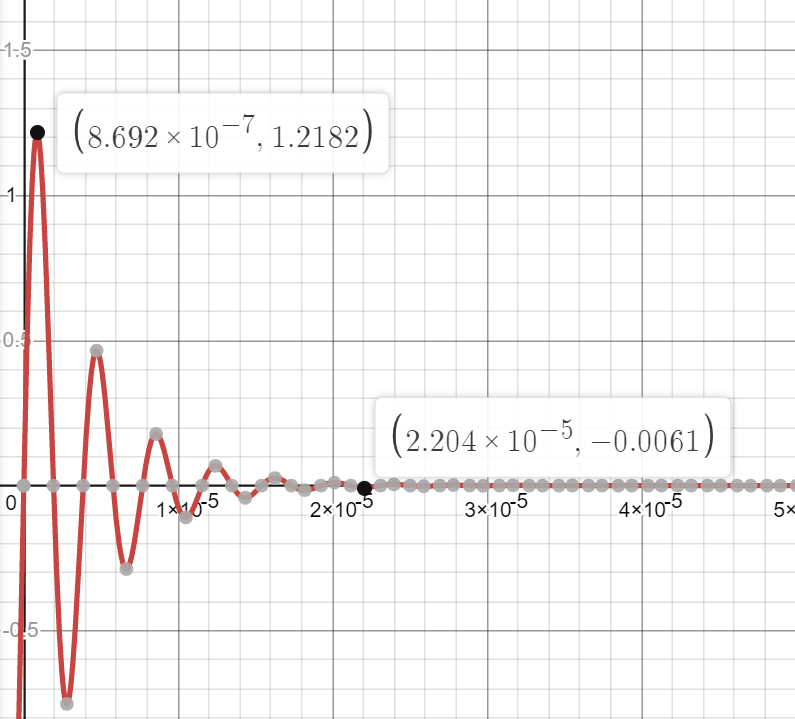
\includegraphics[width=3in]{images/Function_Graph.png}
	\end{figure}
	\subsection*{Error Analysis}
	The error analysis will show that our experimental values and our simulated values match closely with our calculated values. The measured values for the parts used were fine-tuned with the [    ] tool to get measured values were: 1000 ohm resistor (0\% error), 2010 pF capacitor (0.5\%) and a 219 uH inductor (0.5\%). Our frequency from the signal generator was at about 10 kHz. 
	The amplitude of our Voltage waveform from our physical components on the oscilliscope shows 1.249 V on the first peak, whereas the graph used from the calulated values shows 1.218 V for the first peak (2.55\% error). 
	Our sources of error were due mostly to the non-ideal components themselves, even after we had fine-tuned them as close as possible to the values specified. Another source of error would be due to the signal generator outputting a non-ideal square wave. The generator had distortion in the square wave output, rounding off the corners slightly and not having a perfectly vertical line.  
	\subsection*{Conclusion}
	The lab was performed without issue. We were able to successfully calculate, simulate and build the circuit. Our results from each were very similar in each case with very little error.  
\end{document}
